\documentclass[
    notheorems,
    11pt,
    compress,
    aspectratio=169
]{beamer}

\mode<presentation>{
    \usetheme{Madrid}
    \usecolortheme{orchid}
    \usefonttheme[onlymath]{serif}
    \setbeamertemplate{blocks}[rounded][shadow=true]
    \setbeamertemplate{navigation symbols}{}
    \setbeamertemplate{enumerate items}[square]
}

\usepackage{config}

\graphicspath{{./figures/}}
\bibliography{bibliography.bib}

% -----

\title[Agile Methodology]{Software development methodologies}
\subtitle{Agile Methodology}
\author{prof. Leonardo Essam Dei Rossi}
\institute[]{ITT "M. Buonarroti" - Trento (TN)}
\date[A.S. 2025/2026]{Anno scolastico 2025/2026}

% -----

\begin{document}

\setlength{\baselineskip}{15pt}

\begin{frame}
\titlepage
\end{frame}

\begin{frame}
    \frametitle{Indice}

    \tableofcontents
\end{frame}

% -----

\section{What is the Agile methodology?}

\begin{frame}{What is the Agile methodology? (1)}
    The Agile methodology is an approach that divides work into phases, emphasizing continuous delivery and improvement. Agile benefits teams by enabling adaptive planning, rapid execution, and ongoing evaluation, leading to more responsive and successful outcomes.

    \pause
    \vspace{0.5cm}

    The traditional "waterfall" approach has each team work on a project separately, then hand it off to the next group. On the other hand, agile utilizes collaborative, cross-functional teams, emphasizes open communication, teamwork, adaptability, and trust.
\end{frame}

\begin{frame}{What is the Agile methodology? (2)}
    Although the project lead or product owner typically prioritizes the work to be delivered, the team takes the lead on deciding how the work will get done, self-organizing around granular tasks and assignments. Agile isn't defined by a set of ceremonies or specific development techniques.

    \pause
    \vspace{0.5cm}

    Instead, agile is a group of methodologies that demonstrate a commitment to tight feedback cycles and continuous improvement. The original Agile Manifesto didn't prescribe two-week iterations or an ideal team size.
\end{frame}

% -----

\subsection{Key Takeaways}

\begin{frame}{Key Takeaways}
    \begin{itemize}
        \item Agile is a flexible, iterative approach to project management that emphasizes collaboration, continuous delivery, and adaptability;
        \pause
        \item It values people, customer feedback, and working solutions over rigid processes and documentation;
        \pause
        \item Teams tailor Agile practices to their needs, blending frameworks like Scrum and Kanban for optimal results;
        \pause
        \item Experiment with Agile practices and regularly review their effectiveness to foster continuous improvement and team collaboration.
    \end{itemize}
\end{frame}

% -----

\section{Why choose Agile?}

\begin{frame}{Why choose agile? (1)}
    Teams choose agile methodologies so they can respond to changes in the marketplace or customer feedback quickly, without derailing a year's worth of plans. "Just enough" planning and shipping in small, frequent increments lets your team gather feedback on each change and integrate it into future plans at minimal cost.

    \pause
    \vspace{0.5cm}

    But it's not just a numbers game-first and foremost, it's about people. As described by the Agile Manifesto, authentic human interactions are more important than rigid processes.
\end{frame}

\begin{frame}{Why choose agile? (2)}
    Collaborating with customers and teammates is more important than predefined arrangements. Delivering a working solution to the customer's problem is more important than providing hyper-detailed documentation.

    \pause
    \vspace{0.5cm}

    An agile team unites under a shared vision, then brings it to life the way they know is best. Each team sets its own standards for quality, usability, and completeness.
\end{frame}

% -----

\section{The phases of Agile}

\begin{frame}{The phases of Agile}
    \begin{figure}
        \centering
            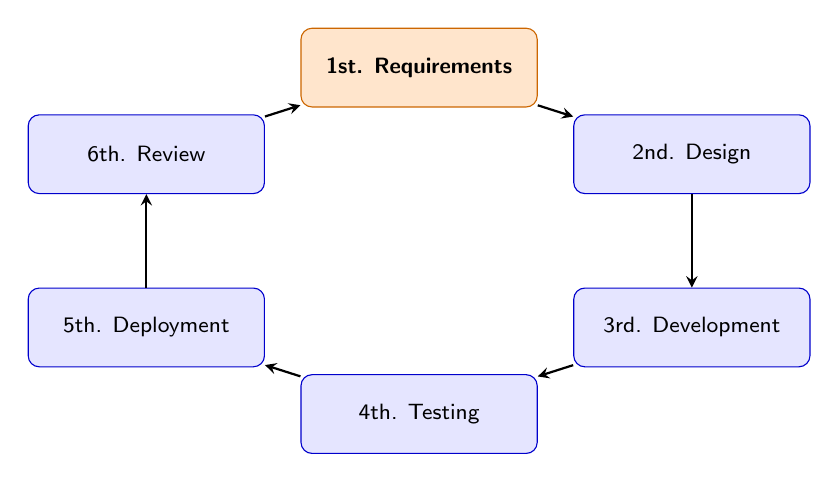
\begin{tikzpicture}[
                box/.style={
                    draw=blue!80!black,
                    fill=blue!10,
                    rectangle,
                    rounded corners,
                    minimum width=3cm,
                    minimum height=1cm,
                    align=center,
                    font=\sffamily\footnotesize
                },
                highlightbox1/.style={
                    box,
                    fill=green!20,
                    draw=green!80!black,
                    text=black
                },
                highlightbox2/.style={
                    box,
                    fill=orange!20,
                    draw=orange!80!black,
                    text=black
                },
                arrow/.style={
                    ->,
                    thick,
                    >=stealth
                }
            ]
    
                \node[highlightbox2] (step1) at (90:4cm and 2.2cm)  {\textbf{1st. Requirements}};
                \node[box] (step2) at (30:4cm and 2.2cm)  {2nd. Design};
                \node[box] (step3) at (330:4cm and 2.2cm) {3rd. Development};
                \node[box] (step4) at (270:4cm and 2.2cm) {4th. Testing};
                \node[box] (step5) at (210:4cm and 2.2cm) {5th. Deployment};
                \node[box] (step6) at (150:4cm and 2.2cm) {6th. Review};
            
                \draw[arrow] (step1) -- (step2);
                \draw[arrow] (step2) -- (step3);
                \draw[arrow] (step3) -- (step4);
                \draw[arrow] (step4) -- (step5);
                \draw[arrow] (step5) -- (step6);
                \draw[arrow] (step6) -- (step1);
        \end{tikzpicture}
    \end{figure}
\end{frame}

% -----

\subsection{Phase \#1: Requirements}

\begin{frame}{Phase \#1: Requirements}
    \begin{block}{}
        In the Waterfall model, requirements are a "signed-and-sealed" contract. In Agile, they are a conversation.
    \end{block}
    
    \pause
    \vspace{0.25cm}
    
    We move away from rigid documentation toward a \textbf{Product Backlog} -- a prioritized list of user needs.

    \vspace{0.25cm}
    
    This phase is about understanding the intent behind a feature rather than just a checklist of technical specs. By focusing on "User Stories", the team remains outcome-oriented, allowing the requirements to evolve as market conditions or user feedback change.
\end{frame}

% -----

\begin{frame}{The phases of Agile}
    \begin{figure}
        \centering
            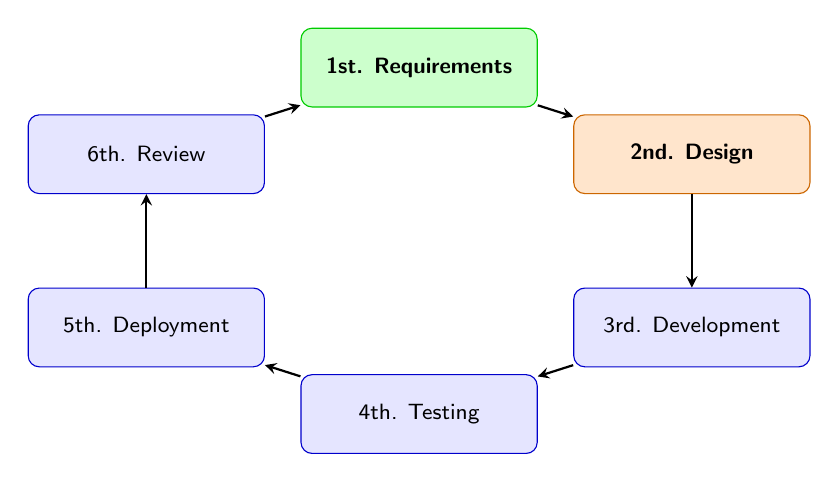
\begin{tikzpicture}[
                box/.style={
                    draw=blue!80!black,
                    fill=blue!10,
                    rectangle,
                    rounded corners,
                    minimum width=3cm,
                    minimum height=1cm,
                    align=center,
                    font=\sffamily\footnotesize
                },
                highlightbox1/.style={
                    box,
                    fill=green!20,
                    draw=green!80!black,
                    text=black
                },
                highlightbox2/.style={
                    box,
                    fill=orange!20,
                    draw=orange!80!black,
                    text=black
                },
                arrow/.style={
                    ->,
                    thick,
                    >=stealth
                }
            ]
    
                \node[highlightbox1] (step1) at (90:4cm and 2.2cm)  {\textbf{1st. Requirements}};
                \node[highlightbox2] (step2) at (30:4cm and 2.2cm)  {\textbf{2nd. Design}};
                \node[box] (step3) at (330:4cm and 2.2cm) {3rd. Development};
                \node[box] (step4) at (270:4cm and 2.2cm) {4th. Testing};
                \node[box] (step5) at (210:4cm and 2.2cm) {5th. Deployment};
                \node[box] (step6) at (150:4cm and 2.2cm) {6th. Review};
            
                \draw[arrow] (step1) -- (step2);
                \draw[arrow] (step2) -- (step3);
                \draw[arrow] (step3) -- (step4);
                \draw[arrow] (step4) -- (step5);
                \draw[arrow] (step5) -- (step6);
                \draw[arrow] (step6) -- (step1);
        \end{tikzpicture}
    \end{figure}
\end{frame}

% -----

\subsection{Phase \#2: Design}

\begin{frame}{Phase \#2: Design}
    \textbf{Agile design rejects the "Big Design Up Front" (BDUF) philosophy.}

    \vspace{0.25cm}
    
    Instead, it favors evolutionary architecture. The team spends enough time to ensure the system is scalable and user-friendly, but they don't try to solve every problem that might occur three years from now. The goal is to create a flexible blueprint that allows for technical pivots without needing to scrap months of planning.
\end{frame}

% -----

\begin{frame}{The phases of Agile}
    \begin{figure}
        \centering
            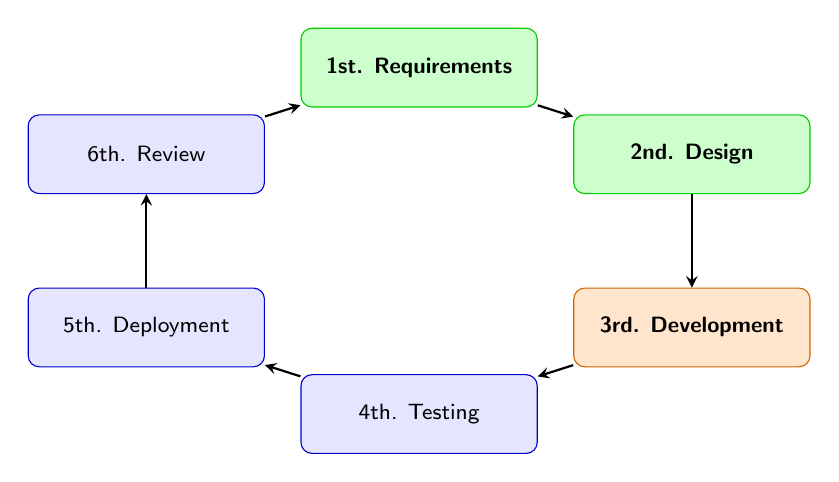
\begin{tikzpicture}[
                box/.style={
                    draw=blue!80!black,
                    fill=blue!10,
                    rectangle,
                    rounded corners,
                    minimum width=3cm,
                    minimum height=1cm,
                    align=center,
                    font=\sffamily\footnotesize
                },
                highlightbox1/.style={
                    box,
                    fill=green!20,
                    draw=green!80!black,
                    text=black
                },
                highlightbox2/.style={
                    box,
                    fill=orange!20,
                    draw=orange!80!black,
                    text=black
                },
                arrow/.style={
                    ->,
                    thick,
                    >=stealth
                }
            ]
    
                \node[highlightbox1] (step1) at (90:4cm and 2.2cm)  {\textbf{1st. Requirements}};
                \node[highlightbox1] (step2) at (30:4cm and 2.2cm)  {\textbf{2nd. Design}};
                \node[highlightbox2] (step3) at (330:4cm and 2.2cm) {\textbf{3rd. Development}};
                \node[box] (step4) at (270:4cm and 2.2cm) {4th. Testing};
                \node[box] (step5) at (210:4cm and 2.2cm) {5th. Deployment};
                \node[box] (step6) at (150:4cm and 2.2cm) {6th. Review};
            
                \draw[arrow] (step1) -- (step2);
                \draw[arrow] (step2) -- (step3);
                \draw[arrow] (step3) -- (step4);
                \draw[arrow] (step4) -- (step5);
                \draw[arrow] (step5) -- (step6);
                \draw[arrow] (step6) -- (step1);
        \end{tikzpicture}
    \end{figure}
\end{frame}

% -----

\subsection{Phase \#3: Development}

\begin{frame}{Phase \#3: Development}
    \textbf{This is the "engine room" of the cycle.}

    \vspace{0.25cm}
    
    Development is broken into short, focused bursts (\textit{sprints}). Rather than building the entire system at once, developers focus on creating a \textbf{Potentially Shippable Product Increment} (PSPI). This ensures that even if the project were halted tomorrow, the team would still have a functional piece of software to show for their efforts.

    \pause
    \vspace{0.25cm}
    
    \begin{block}{}
        It’s an approach that prioritizes "working software over comprehensive documentation".
    \end{block}
\end{frame}

% -----

\begin{frame}{The phases of Agile}
    \begin{figure}
        \centering
            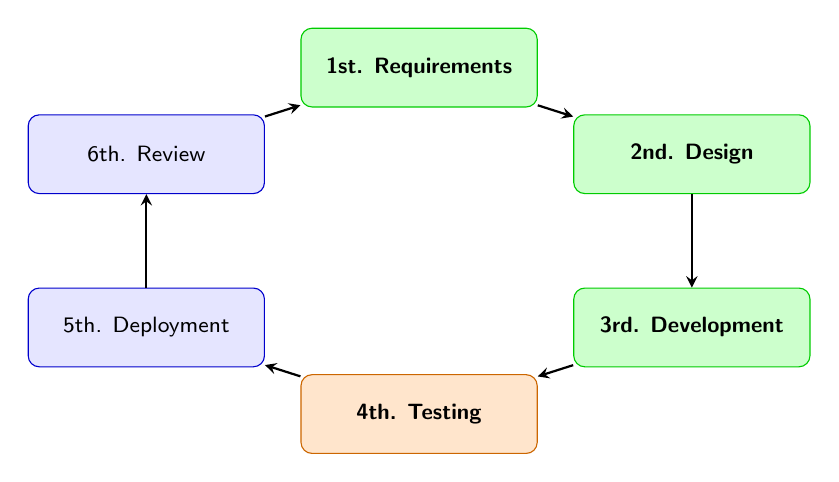
\begin{tikzpicture}[
                box/.style={
                    draw=blue!80!black,
                    fill=blue!10,
                    rectangle,
                    rounded corners,
                    minimum width=3cm,
                    minimum height=1cm,
                    align=center,
                    font=\sffamily\footnotesize
                },
                highlightbox1/.style={
                    box,
                    fill=green!20,
                    draw=green!80!black,
                    text=black
                },
                highlightbox2/.style={
                    box,
                    fill=orange!20,
                    draw=orange!80!black,
                    text=black
                },
                arrow/.style={
                    ->,
                    thick,
                    >=stealth
                }
            ]
    
                \node[highlightbox1] (step1) at (90:4cm and 2.2cm)  {\textbf{1st. Requirements}};
                \node[highlightbox1] (step2) at (30:4cm and 2.2cm)  {\textbf{2nd. Design}};
                \node[highlightbox1] (step3) at (330:4cm and 2.2cm) {\textbf{3rd. Development}};
                \node[highlightbox2] (step4) at (270:4cm and 2.2cm) {\textbf{4th. Testing}};
                \node[box] (step5) at (210:4cm and 2.2cm) {5th. Deployment};
                \node[box] (step6) at (150:4cm and 2.2cm) {6th. Review};
            
                \draw[arrow] (step1) -- (step2);
                \draw[arrow] (step2) -- (step3);
                \draw[arrow] (step3) -- (step4);
                \draw[arrow] (step4) -- (step5);
                \draw[arrow] (step5) -- (step6);
                \draw[arrow] (step6) -- (step1);
        \end{tikzpicture}
    \end{figure}
\end{frame}

% -----

\subsection{Phase \#4: Testing}

\begin{frame}{Phase \#4: Testing}
    \textbf{Testing in Agile is not a "gate" at the end of a project, it is woven into the very fabric of development.}

    \vspace{0.25cm}
    
    By implementing \textit{Continuous Testing} \cite{enwiki:1329392723} and automated suites, the team ensures that new features don't break existing functionality. This shift-left approach means bugs are caught while the code is still fresh in the developer's mind, drastically reducing the cost and time of repairs.
\end{frame}

% -----

\begin{frame}{The phases of Agile}
    \begin{figure}
        \centering
            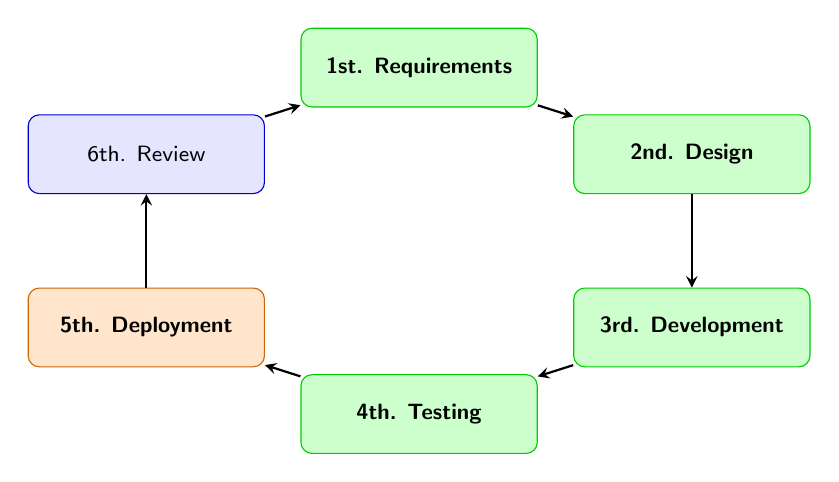
\begin{tikzpicture}[
                box/.style={
                    draw=blue!80!black,
                    fill=blue!10,
                    rectangle,
                    rounded corners,
                    minimum width=3cm,
                    minimum height=1cm,
                    align=center,
                    font=\sffamily\footnotesize
                },
                highlightbox1/.style={
                    box,
                    fill=green!20,
                    draw=green!80!black,
                    text=black
                },
                highlightbox2/.style={
                    box,
                    fill=orange!20,
                    draw=orange!80!black,
                    text=black
                },
                arrow/.style={
                    ->,
                    thick,
                    >=stealth
                }
            ]
    
                \node[highlightbox1] (step1) at (90:4cm and 2.2cm)  {\textbf{1st. Requirements}};
                \node[highlightbox1] (step2) at (30:4cm and 2.2cm)  {\textbf{2nd. Design}};
                \node[highlightbox1] (step3) at (330:4cm and 2.2cm) {\textbf{3rd. Development}};
                \node[highlightbox1] (step4) at (270:4cm and 2.2cm) {\textbf{4th. Testing}};
                \node[highlightbox2] (step5) at (210:4cm and 2.2cm) {\textbf{5th. Deployment}};
                \node[box] (step6) at (150:4cm and 2.2cm) {6th. Review};
            
                \draw[arrow] (step1) -- (step2);
                \draw[arrow] (step2) -- (step3);
                \draw[arrow] (step3) -- (step4);
                \draw[arrow] (step4) -- (step5);
                \draw[arrow] (step5) -- (step6);
                \draw[arrow] (step6) -- (step1);
        \end{tikzpicture}
    \end{figure}
\end{frame}

% -----

\subsection{Phase \#5: Deployment}

\begin{frame}{Phase \#5: Deployment}
    \textbf{The deployment phase is where the "rubber meets the road".}

    \vspace{0.25cm}
    
    In a mature Agile environment, this often utilizes \textit{Continuous Delivery} \cite{enwiki:1322843384} pipelines. The objective is to get the software into the hands of actual users as quickly and safely as possible. This allows the business to realize value immediately and provides the team with real-world data on how the feature is actually being used.
\end{frame}

% -----

\begin{frame}{The phases of Agile}
    \begin{figure}
        \centering
            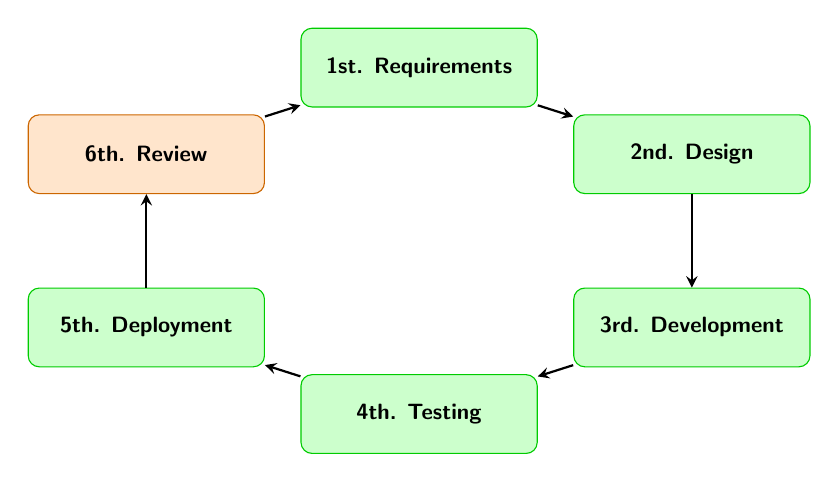
\begin{tikzpicture}[
                box/.style={
                    draw=blue!80!black,
                    fill=blue!10,
                    rectangle,
                    rounded corners,
                    minimum width=3cm,
                    minimum height=1cm,
                    align=center,
                    font=\sffamily\footnotesize
                },
                highlightbox1/.style={
                    box,
                    fill=green!20,
                    draw=green!80!black,
                    text=black
                },
                highlightbox2/.style={
                    box,
                    fill=orange!20,
                    draw=orange!80!black,
                    text=black
                },
                arrow/.style={
                    ->,
                    thick,
                    >=stealth
                }
            ]
    
                \node[highlightbox1] (step1) at (90:4cm and 2.2cm)  {\textbf{1st. Requirements}};
                \node[highlightbox1] (step2) at (30:4cm and 2.2cm)  {\textbf{2nd. Design}};
                \node[highlightbox1] (step3) at (330:4cm and 2.2cm) {\textbf{3rd. Development}};
                \node[highlightbox1] (step4) at (270:4cm and 2.2cm) {\textbf{4th. Testing}};
                \node[highlightbox1] (step5) at (210:4cm and 2.2cm) {\textbf{5th. Deployment}};
                \node[highlightbox2] (step6) at (150:4cm and 2.2cm) {\textbf{6th. Review}};
            
                \draw[arrow] (step1) -- (step2);
                \draw[arrow] (step2) -- (step3);
                \draw[arrow] (step3) -- (step4);
                \draw[arrow] (step4) -- (step5);
                \draw[arrow] (step5) -- (step6);
                \draw[arrow] (step6) -- (step1);
        \end{tikzpicture}
    \end{figure}
\end{frame}

% -----

\subsection{Phase \#6: Review}

\begin{frame}{Phase \#6: Review}
    The final phase is perhaps the most critical for the Agile philosophy of "inspect and adapt":

    \vspace{0.25cm}

    \begin{itemize}
        \item \textbf{The Sprint Review:}\\brings in stakeholders to validate that the team is building the right thing;

        \item \textbf{The Retrospective:}\\allows the team to look inward to ensure they are building it the right way.
    \end{itemize}

    \vspace{0.25cm}
    \pause

    \begin{block}{}
        This isn't just a wrap-up; it's the bridge to the next cycle, ensuring that every mistake becomes a lesson for the next iteration.
    \end{block}
\end{frame}

% -----

\section{Agile vs. Waterfall}

\begin{frame}{Agile vs. Waterfall (1)}
    Agile was first adopted by software teams, who moved from the traditional, sequential waterfall approach to a method that garnered consistent feedback and adjustment throughout the development lifecycle.

    \pause
    \vspace{0.5cm}

    Agile project management takes an iterative approach to development by creating several incremental steps with regular feedback intervals. This promotes adaptability since a team can adjust throughout the product development process, rather than being confined to a linear path. It also allows for regular, high-impact releases that enable teams to deliver a series of wins over time.
\end{frame}

\begin{frame}{Agile vs. Waterfall (2)}
    Iterative releases unlock multiple opportunities for a team to:

    \begin{itemize}
        \item Adapt to changing circumstances from newly discovered requirements to a blocked piece of work;
        \pause
        \item Gather feedback from stakeholders during the process and iterate responsively without the stress of a final delivery deadline;
        \pause
        \item Build relationships and connections across roles that make it easier for people to connect and communicate effectively.
    \end{itemize}

    \vspace{0.5cm}

    \pause
    Agile allows teams to be more resilient to changes that inevitably occur during a project.
\end{frame}

%\begin{frame}[fragile]
%    \frametitle{Agile vs. Waterfall (3)}
%
%    \begin{figure}
%        \centering
%        \includesvg[scale=0.8]{assets/fig01-agileschema.svg}
%        \caption{Agile cycle (1).}
%    \end{figure}
%\end{frame}

% -----

\begin{frame}{Riferimenti e approfondimenti}
    \printbibliography
\end{frame}

% -----

\end{document}
